\chapter{Problem sterowania robotem społecznym}

\section{Agent mobilny}
Słownik języka polskiego nie definiuje słowa agent w takim rozumieniu, w jakim będzie ono używane w poniższej pracy, ponieważ jest to zapożyczenie z języków obcych. Jedna z definicji oksfordzkiego słownika języka angielskiego mówi: \textit{"A person or thing that takes an active role or produces a specified effect"}, co można przetłumaczyć jako \textit{"Osoba lub rzecz, która bierze udział lub przyczynia się do realizacji określonego efektu"}. 

Pojęcie agenta pochodzi z informatyki, gdzie oznacza autonomiczny program realizujący zadanie, np. zbieranie i przetwarzanie informacji.
Najłatwiej jest opisać agenta jako obiekt (w rozumieniu programowania obiektowego). Obiekty składają się pól i posiadają metody. Dostęp do zawartości pól i do wywoływania metod może być ograniczany (prywatny) lub ogólnie dostępny (publiczny), ale decyzja o podjęciu przez obiekt jakiegoś działania delegowana jest do wyższych warstw programu, np. nadrzędnej funkcji lub programisty wywołującego metodę z poziomu linii komend. 

Cechą wyróżniającą agentów od pozostałych obiektów jest autonomiczność. Agent na podstawie swojego stanu lub wiedzy o świecie może samodzielnie zdecydować o podjęciu działania. Pojęcie agenta przeszło z informatyki do robotyki, gdzie jest rozumiane jako obiekt przekształcający percepcję na inteligentne działanie. Robot jest agentem uprzedmiotowionym, czyli posiadającym fizyczną formę i oddziałującym z realnym światem.

\subsection{Klasyfikacja CERT}

%\begin{wraptable}{p}{0.5\linewidth}
%\caption{Typy agentów}
%\label{tab:cert}
%\begin{tabular}{ | l | p{6cm} | } \hline
%C & zbyt prymitywny do realizacji jakiegokolwiek zadania \\ \hline
%CE  & mogący jedynie oddziaływać na otoczenie \\ \hline
%CR & jedynie gromadzący dane \\ \hline
%CT & zdolny do komunikacji, mogący przetwarzać dane, "serwer", "obliczenia w chmurze" \\ \hline
%CER & agent niezależny \\ \hline
%CET & zdalny efektor  \\ \hline
%CRT & zdalny czujnik \\ \hline
%CERT & kompletny agent \\ 
%\hline
%\end{tabular}
%\end{wraptable} 

W pracy \cite{ZIEL} przedstawiono osiem typów agentów, podzielonych ze względu na komponenty wchodzące w ich skład. Możemy wyróżnić cztery podsystemy: sterowania (C), stanowiący podstawowy element struktury agenta; efektorów (E), oddziałowujący na otoczenie; receptorów (R), zbierający informacje o stanie otoczenia; oraz komunikacji (T), pozwalający na bezpośrednią wymianę informacji z innymi agentami. Podsystem sterowania jest niezbędny, podczas gdy pozostałe są opcjonalne. Pozwala to utworzyć klasyfikację, ze względu na posiadane podsystemy. % Typy agentów opisano w tabeli 2.1. % \ref{tab:cert}. 

\textcolor{red}{W środowisku wieloagentowym podsystem komunikacji pełni kluczową rolę. Robot społeczny musi być zdolny do tworzenia społeczności, a więc nadawać i odbierać informacje. Struktura podsystemów agenta może być stała, lub zmienna. Niedoścignionym wzorem dla projektantów robotów są organizmy żywe charakteryzujące się zdolnością do adaptacji do zmiennych warunków środowiska i poszerzania swoich możliwości dzięki wymianie informacji.}

\subsection{Klasyfikacja ze względu na podsystem sterowania}

Ze względu na sposób działania podsystemu C można wyróżnić \textbf{agentów czysto reaktywnych}, którzy reagują na aktualny stan świata, oraz \textbf{agentów z parametrem wewnętrznym}, analizujących również poprzednie stany świata. \cite{GNAT}

\subsubsection{Agent czysto reaktywny}

Działanie podsystemów R oraz E można zamodelować przy pomocy dwóch funkcji: \textit{see()} zwracającej stan świata, oraz \textit{action()} oddziałującej na świat. Zadaniem podsystemu sterowania jest przetworzyć wyjście funkcji \textit{see()} na wejście funkcji \textit{action()}. Opisywany agent zrealizuje zadanie bezpośrednio, przetwarzając dane ad hoc.

\subsubsection{Agent z parametrem wewnętrznym}

Agent realizuje zadanie na podstawie wygenerowanych modeli świata. Modele te są przechowane w bazie danych. Oprócz podsystemów E i R modelowany jest również podsystemów C przy u użyciu funkcji \textit{next()} która wywołana jest na dwa sposoby. Argumentem tej funkcji mogą być informacje z otoczenia (wyjście funkcji \textit{see()}). Agent tworzy wtedy aktualny model świata. Argumentem może być również para: istniejący już model i jedna z dostępnych akcji. Pozwala to na przewidywanie konsekwencji akcji i tworzenie planów. 

Działanie agentów z parametrem wewnętrznym może być traktowane jako podróż po grafie skierowanym, którego wierzchołkami są różne modele świata, a krawędziami dostępne akcje. Planowanie działań sprowadza się do wyznaczenia ścieżki między początkowym a końcowym stanem świata.

\section{Model BDI}
Model belief-desire–intention (przekonań-pragnień-intencji) to metodyka projektowania agentów skoncentrowana na odtworzeniu bardzo uproszczonego schematu ludzkiego działania. Schemat został opracowany przez filozofa Michaela Bratmana i jest wykorzystywany w informatyce. Człowiek motywowany jest do aktywności poprzez potrzeby lub marzenia. Potrafi on wyobrazić sobie docelowy stan otaczającego go świata, a następnie określić plan który do niego doprowadzi. Plan jest dekomponowany na podzadania, które realizowane są w ustalonej kolejności. Plan może zostać przeformułowany, aby dostosować się do zmian otoczenia.

Działanie modelu BDI skoncentrowane jest na realizacji celu. Zasadność wyboru akurat przekonań, pragnień i intencji jest omawiana w pracy \cite{RAO}. Określone są tam również wymagania, które musi spełniać implementacja modelu BDI.

Agent działa w czasie rzeczywistym, w dynamicznym środowisku, zmieniającym się nie tylko na skutek jego działań. Świat może zmieniać się spontanicznie, lub w efekcie działań innych obiektów. Osiągnięcie zadania wymaga więc elastycznego planu. Reagując na zmiany, agent musi aktualizować sekwencję akcji, więc sam w sobie jest niedeterministyczny. Agent może mieć jednocześnie kilka zadań, które musi skutecznie priorytetyzować lub nawet w skrajnych przypadkach porzucać niektóre z nich. % a w skrajnych przypadkach umieć rezygnować niektórych z nich.

BDI musi umożliwiać tworzenie modelu świata i pozwalać na przewidywanie potencjalnych zmian. Agent BDI posiadając pamięć i estymując przyszłe parametry świata może planować zachowanie w sposób bardziej skomplikowany, niż agent z parametrem wewnętrznym. Wierzchołki (stany świata) wspomnianego wcześniej grafu mogą być połączone nie tylko dostępnymi dla agenta akcjami, ale również niezależnymi od jego działań zdarzeniami. Powinny być one uwzględnione przy generowaniu planu.

W modelu wyróżnia się trzy kluczowe elementy podsystemu sterowania agenta, opisane poniżej. 

\subsubsection{Przekonania}
Opisują stan świata postrzegany przez agenta. Używa się słowa "przekonania", a nie "wiedza" dla pokreślenia, że agent może wierzyć w zdania, które niekoniecznie są prawdziwe. Dzięki regułom wnioskowania możliwe jest estymowanie zmian i lepsze dostosowanie się do środowiska. 

\subsubsection{Pragnienia}
Opisują stan świata pożądany przez agenta. Mogą być definiowane w ogólny sposób, na przykład "bądź szczęśliwy", "kultywuj przyjaźń",

Pragnienia urzeczywistniają się poprzez stawianie sobie celów. Pragnienie może być zdefiniowane ogólnie, natomiast cel musi określać warunki sukcesu. Pragnienia mogą być sprzeczne, więc agent może wyznaczać sobie wiele sprzecznych celów. 

{\subsubsection{Intencje}
Opisują hierarchię pragnień agenta. Agent określa cele, które zobowiązuje się wykonać i przechodzi do ich realizacji. \\}

% Planner, 
% system emocji
% pamięć

% model symuluje zachowanie człowieka

Model BDI posiadając pamięć i estymując przyszłe parametry świata może planować zachowanie rozumiane jako podróż po grafie nie tylko na podstawie akcji. Stany świata mogą zmieniać się spontanicznie, więc one również powinny zostać uwzględnione. 
% krawędzie action() i krawędzie chance()

\section{Robot społeczny}
Robot społeczny, to uprzedmiotowiony agent zdolny do funkcjonowania w środowisku ludzi, w szczególności tworzenia relacji, wyrażania emocji oraz realizowania innych wysokopoziomowych kompetencji społecznych. Uprzedmiotowiony, to jest posiadający fizyczną formę (awatara), stanowiącą interfejs pomiędzy agentem (umysłem), a światem rzeczywistym. 

\subsection{Architektura robota społecznego jako agenta CERT}

Ponieważ agent posiada swojego awatara, dokonujemy rozróżnienia pomiędzy receptorami i efektorami rzeczywistymi oraz wirtualnymi. Rzeczywiste oddziałują ze światem fizycznym, obierając i generując bodźce takie jak dotyk, dźwięk lub obraz. Traktujemy je jako niskopoziomowe elementy architektury. Receptory i efektory wirtualne pozwalają na realizację bardziej skomplikowanych działań, takich jak rozpoznawanie twarzy, śledzenie obiektu czy ekspresję emocji. Kompetencje te jednak są pozbawione charakteru społecznego, ponieważ same w sobie są bezkontekstowe i niezorientowane na cel – stanowią warstwę pośrednią.

Ludzie nie mają możliwości w intuicyjny sposób na oddziaływanie z podsystemem komunikacji między agentowej. Podsystem T bezpośrednio nie poszerza kompetencji społecznych, ale służy do zlecania zdalnych obliczeń, pobierania danych ze zdalnych baz. Aby być zrozumiałym dla człowieka agent swoje działania powinien wyrażać poprzez podsystem E, wpływając na świat rzeczywisty. 

Obiektem zainteresowania robota są ludzie lub inne roboty. Jego cele koncentrują się na wejściu w interakcje. Człowiek jako istota empatyczna przypisuje robotowi często większe możliwości, niż te, do których robot jest zdolny. Gdy okazuje się, że robot jest bezkontekstowy (gdy rozmówca odkryje, że zasadą działania się proste warunki, a nie motywacje lub marzenia) szybko przestaje być obiektem zainteresowania. Dlatego kluczowym elementem architektury jest podsystem sterowania, który musi zawierać w sobie model umysłu imitujący ludzki. 

\subsection{Cechy robota społecznego}

W pracy \cite{FONG} % (Fonga, Nourbakhsha i Dautenhahna) 
wymieniono siedem cech robota społecznego:
\begin{itemize}
    \setlength\itemsep{-0.4em}
    \item wyrażanie i postrzeganie emocji;
    \item zdolność do wysokopoziomowej komunikacji werbalnej; 
    \item wykorzystywanie naturalnych gestów, "mowy ciała", do komunikacji niewerbalnej;
    \item rozpoznawanie i zapamiętywanie innych agentów, lub ludzi;
    \item nawiązywanie i utrzymywanie relacji społecznych;
    \item posiadanie własnego charakteru i cech osobowości;
    \item zdolność do nauki i rozwijania umiejętności społecznych.
\end{itemize}

W obecnej chwili nie istnieje żaden robot, który spełniałby wszystkie te warunki.
% Działa deliberatywnie – cyklicznie wykonuje trzy działania: odczuwa, planuje i działa.

%  (agent upostaciowiony robot - embodied agents)

\section{Robot NAO}

\begin{wrapfigure}{p}{0.29\textwidth}
    \centering
    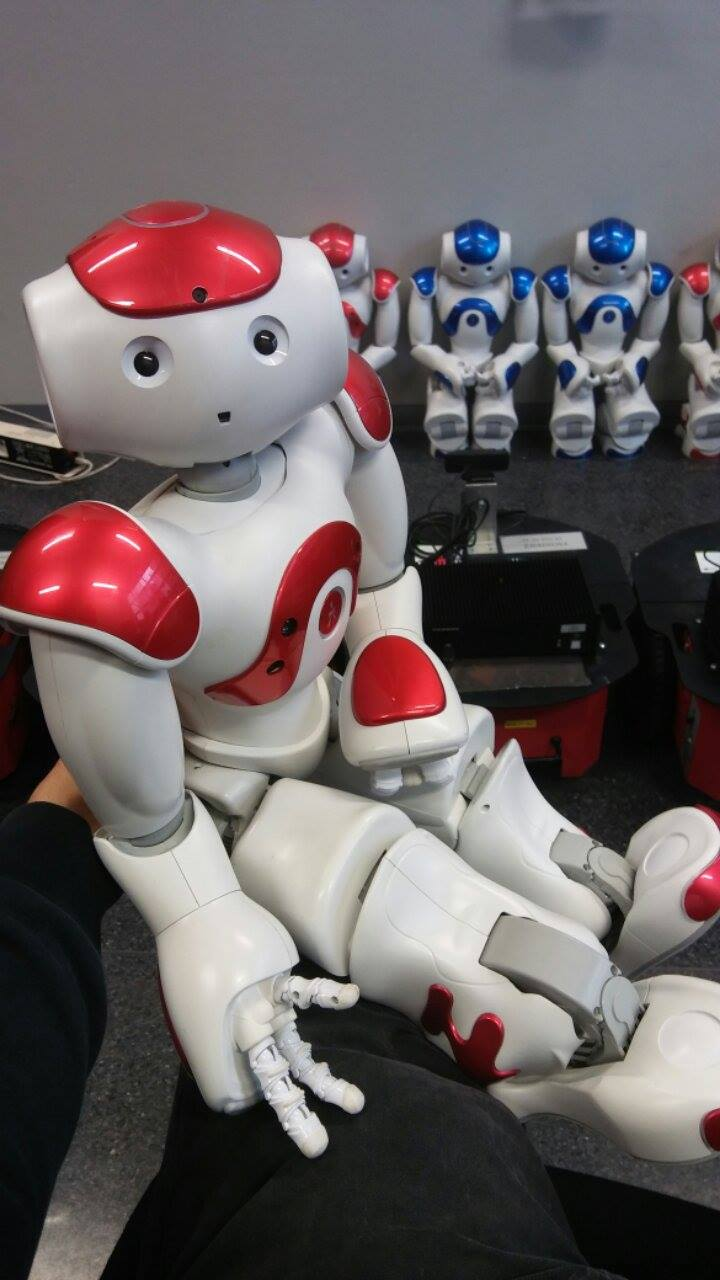
\includegraphics[width=0.25\textwidth]{images/nao.jpg}
    \caption{Robot NAO}
\end{wrapfigure}

Robot NAO to mały robot humanoidalny. Został stworzony przez firmę Aldebaran Robotics na użytek uczelni wyższych oraz ośrodków naukowych do badań nad robotyką społeczną i interakcją człowiek-robot. Przykładem takich badań są zawody RoboCup, gdzie drużyny złożone z 4 NAO grają przeciwko innym drużynom w uproszczoną wersję piłki nożnej. 

Robot pracuje na systemie operacyjnym NAOqi, monitorującym jego stan działania, pozwalającym na realizację
Producent udostępnia bogate biblioteki dające dostęp do wielu kompetencji robota. Z punktu widzenia osoby chcącej zaprogramować scenariusz działania robota można dokonać podziału kompetencji na dwie kategorie: 
\begin{itemize}
    \setlength\itemsep{-0.4em}
    \item niskopoziomową, mechaniczną, związaną z geometrią, dynamiką i czujnikami robota, pozwalającą na przykład na wydawanie komend silnikom, odczyt sygnałów z mikrofonu, kamer lub siłomierzy, czy zmianę koloru diód umieszczonych przy oczach; 
    \item wysokopoziomową, programową, realizującą zaawansowane algorytmy, takie jak rozpoznanie mowy, lub twarzy, śledzenie obiektu (wodzenie za nim wzrokiem), czy zmianę pozycji i przemieszczenie się do innego miejsca. 
\end{itemize}

\subsection{NAO jako agent CERT}

Możemy wspominaną warstwę niskopoziomową potraktować jako receptory i efektory rzeczywiste. Nie pozwalają one bezpośrednio na realizację scenariuszy społecznych, ponieważ nie udostępniają środków do uogólnienia wiedzy, ani nie modelują umysłu. 

Warstwa wysokopoziomowa będzie traktowana jako wirtualne podsystemy E i R. Znacząco rozszerza możliwości robota, dostarczając wyższych warstw abstrakcji, ułatwiając pracę programiście i pozwalając na interakcję z człowiekiem. Niestety taka interakcja okazuje się płytka i bezosobowa. Dla przykładu robot potrafi śledzić twarz, jednak nie przypisuje jej konkretnej osobie, ponieważ nie ma jak jej rozpoznać i zapamiętać.

\subsection{NAO jako robot społeczny}

Za realizację scenariuszy działania odpowiada podsystem sterowania. Domyślnie po uruchomieniu, bez ingerencji użytkownika, NAO jest jedynie prymitywnym konstruktem cechującym się podstawową responsywnością bazującą na sygnałach odbieranych z wirtualnych receptorów i przekuwanych w odpowiedź przy wykorzystaniu wirtualnych efektorów. Jego działania sprowadzają sie do przestępowanią z nogi na nogę, ruchów przypominających oddech oraz podążaniu wzrokiem za twarzą. Tworzone scenariusze są zazwyczaj bardzo proste i nie modelują umysłu. NAO nie jest zdolny do podjęcia wysokopoziomowej interacji, nie posiada emocji, ani nie zapamiętuje osób przebywających w jego otoczeniu, więc nie spełnia wymagań stawianych robotom społecznym.

